\documentclass[a4paper,11pt]{article}
\usepackage{layout}
\usepackage{lscape}
\usepackage[utf8]{inputenc}
\usepackage{a4wide}
\usepackage[dvips]{graphicx}
\usepackage{url}
\usepackage[colorlinks=true]{hyperref}
\usepackage[table,dvipsnames]{xcolor}[2004/07/04]

\author{Jachym Cepicky}

\title{Implementation of OGC's WPS standard: PyWPS}

\makeatletter
%\Lesejk
\def\Lesejk{{\tt{}Les-e\makebox(2,11)[t]{\rotatebox{35}{j}}\kern-.1667em\lower.5ex\hbox{\rotatebox{315}{k}}\kern-.125em\@}}


\newcommand{\link}[1]{\texttt{<\url{#1}>}}
\newcommand{\pywpssite}{\url{http://pywps.wald.intevation.org}}
\newcommand{\pywpswiki}{\url{http://pywps.ominiverdi.org/wiki}}
\newcommand{\note}[1]{\medskip{}\noindent{}NOTE: #1\medskip{}}
\newcommand{\version}{\emph{2.0.0}}
\makeatother


\pagestyle{plain}

\begin{document}
\maketitle{}

\bigskip
\begin{quote}
    Copyright \copyright  2006 PyWPS Development Team
    Permission is granted to copy, distribute and/or modify this document
    under the terms of the GNU Free Documentation License, Version 1.2
    or any later version published by the Free Software Foundation;
    with no Invariant Sections, no Front-Cover Texts, and no Back-Cover Texts.
    A copy of the license is included in the section entitled "GNU
    Free Documentation License".
\end{quote}
\bigskip


In this file, you can found the description of installation and
configuration of PyWPS script. At the and, you can learn, how to add
your own process. This document describes most recent
version of PyWPS (\version), available in subversion respository.

PyPWS project has been started on April 2006 with support of DBU --
Deutsche Bundesstiftung Umwelt\footnote{\url{http://dbu.de}} and with help of
GDF-Hannover\footnote{\url{http://gdf-hannover.de}} and Help Service Remote
Sensing\footnote{\url{http://www.bnhelp.cz}} companies. Initial author is Jachym
Cepicky\footnote{\url{http://les-ejk.cz}}.
    

    \tableofcontents

\newpage

%---------------------------------------------------------------------
\section{Introduction}
PyWPS (Python Web Processing Service) is implementation of Web
Processing Service 0.4.0 standard from Open Geospatial
Consortium\footnote{\url{http://www.opengeospatial.org/standards/requests/28}}.

It has been started on Mai 2006 as project supported by DBU. It offers
environment for programming own process (geofunctions or models) which can
be accessed from the public. The main advantage of PyWPS is, that it has
been written with native support for GRASS
GIS\footnote{http://grass.itc.it}. Access GRASS modules via web
interace should be as easy as possible.
However, not only GRASS GIS is supported. Usage of other programs, like
R package or GDAL or PROJ tools is possible as well.

PyWPS is written in Python programming language, your processes must use
this language too. 

PyWPS Homepage can be found at \pywpssite.
PyWPS Wiki is hosted on \pywpswiki. 

\subsection{How it works}
PyWPS is an translator application between client (Web Browser, Desktop
GIS, command line tool, \dots) and working tool installed on the server.
PyWPS does no work by it self. As working tool, GRASS GIS, GDAL, PROJ, R
and other programs can be used.

\begin{figure}[ht]
\begin{center}
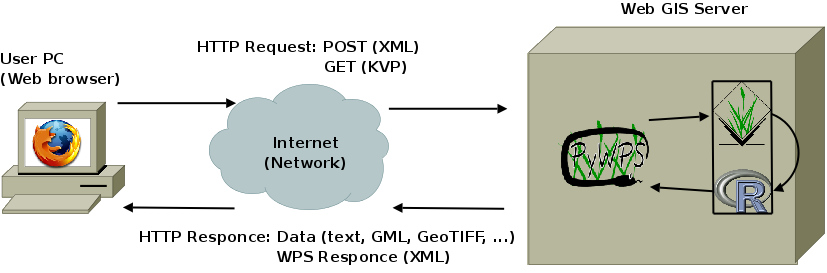
\includegraphics[width=1\textwidth]{pic/pywps-schema}
\caption{How does PyWPS work: GRASS GIS is in this case working tool}
\label{pic:pywps}
\end{center}
\end{figure}

%---------------------------------------------------------------------
\section{Quick install}
\begin{enumerate}
    \item Install PyWPS, see page~\pageref{install} for details
    \item NOTE: Copy original files (process examples, configuration files)
    with \texttt{.py-dist} suffix to \texttt{.py}, when you see them.
    \item Edit configuration files in \texttt{pywps/etc/} directory. See
    page~\pageref{configuration} for details.
    \item Create or edit \texttt{\_\_init\_\_.py} file in
    \texttt{pywps/processes} directory. Add available process names to
    \texttt{\_\_all\_\_} structure.
    \item Add your processes to \texttt{pywps/processes} directory. See
    page~\pageref{processes} for details.
    \item Run PyWPS with \texttt{./wps.py} command, see
    page~\pageref{testing} for details.
\end{enumerate}

    
%---------------------------------------------------------------------
\section{Know issues}
Known bugs and limitations to \date
\begin{itemize}
\item Sometimes, when there is e.g. SyntaxError in the process, teporary file \texttt{/tmp/pywps*} is not deleted, which ledts to \texttt{ServerBussy} exception and the files have to be removed by hand.
\item  If inputs are of type \texttt{LiteralValue} and it's type is
string, it is not controlled properly. Take care on your inputs and do
not use it directly in scripts to avoid your server to be hacked.
\end{itemize}

Please report all problems or unexpected handeling either via pywps mailing
list\footnote{\href{http://wald.intevation.org/mailman/listinfo/pywps-devel}{PyWPS
- development list}}
or using PyWPS
bugtracker\footnote{\href{http://wald.intevation.org/tracker/?atid=174&group\_id=22&func=browse}{PyWPS
Bug tracker}}.

%---------------------------------------------------------------------
\section{Installation}
\label{install}   
Required packages:
    
\begin{itemize}
    \item python 
    \item python-xml 
\end{itemize}
    
Recommended packages:
    
\begin{itemize}
    \item Web Server (e.g. Apache) -- \url{http://httpd.apache.org} -  You
    will need an web server, to be able to execute processes from remote
    computers.

    \item GIS GRASS  -- \url{http://grass.itc.it} - Geographical Resources
    Analysis Support System (GRASS) is Open Source GIS, which provides more
    then 350 modules for raster and vector (2D, 3D) data analysis. PyWPS is
    written with native support for GRASS and it's functions.

    \item PROJ.4  -- \url{http://proj.maptools.org} - Cartographic
    Projections library used in various Open Source projects, such as
    GRASS, UMN MapServer, QGIS and others. It can be used e.g. for data
    transformation.

    \item GDAL/OGR  -- \url{http://gdal.org} - translator library for
    raster geospatial data formats, is used in various projects for
    importing, exporting and transformation between various raster and vector
    data formats.

    \item R  -- \url{http://www.r-project.org} - is a language and environment
    for statistical computing and graphics.

\end{itemize}
    
\subsection{Installation the quick 'n' dirty way}
For installing pywps to your server simply unzip the archive to the
directory, where cgi programs are allowed to run. You can also use current
repository version.

\begin{verbatim}
$ cd /usr/lib/cgi-bin/
$ tar xvzf /tmp/pywps-VERSION.tar.gz
$ pywps/wps.py
\end{verbatim}

\subsection{Installation the 'clean' way}
Unzip the package 
\begin{verbatim}
$ tar -xzf pywps-VERSION.tar.gz
\end{verbatim}
and run 
\begin{verbatim}
$ python setup.py install
\end{verbatim} 

Several binary packages for Linux distributios are also avaliable on PyWPS
homepage\footnote{\pywpssite}.

%---------------------------------------------------------------------
\section{Configuration}
\label{configuration}
    
Before you start to tune your PyWPS installation, you should get your copy of
OpenGIS(R) Web Processing Service document (OGC 05-007r4) version
0.4.0\footnote{\url{http://www.opengeospatial.org/standards/requests/28}}.
    
\note{Note, that the configuration option are CASE SENSITIVE}
    
Pywps configuration takes places in two files. The files are actually python
scripts, so it does not harm, if you have some experience in python
programming language. But you should be able to setup the program without
any python knowledge.

The first file is in \texttt{pywps/etc/settings.py} and (optional) the second file is
\texttt{pywps/etc/grass.py} which has to be setuped if you do want to use
GRASS GIS modules in your scripts. Some special "tuning" can be done in
\texttt{pywps/processes/\_\_init\_\_.py}
file. You can allways obtain original configuration files from
\texttt{pywps/Wps/default\_settings.py} and \texttt{pywps/Wps/default\_grass.py}.
    
\subsection{Main configuration file \texttt{pywps/etc/settings.py}}
    
This file has got two sections: WPS and serverSettings
    
In the \texttt{WPS} section, the main configuration is set, which appears mostly in
GetCapabilities request. The \emph{mandatory} parameters, which should be set up
are (with default/recommend values):
    

\begin{verbatim}
WPS = {
    'version': "0.4.0",
    'encoding': "utf-8",
    'ServiceIdentification': {
        'Title':"Jachym's WPS server",
        'ServiceType':"WPS",
        'ServiceTypeVersion':"0.1.0",
        'Abstract':'Abstract to this WPS',
    },
    'ServiceProvider': {
            'ProviderName' : "Your Company",
            'IndividualName':"Your Name",
            'PositionName':"Your Position",
            'Role':"your role",
            'DeliveryPoint': "Street",
            'City': "City",
            'PostalCode':"00000",
            'Country': "Your country",
            'ElectronicMailAddress':"your.email@address",
    },

    'OperationsMetadata': {
        'ServerAddress' : "http://localhost/cgi-bin/wps/wps.py",
    },
    'Keywords' : ['GRASS','GIS','WPS'],
}
\end{verbatim}

    
In the \texttt{ServerSettings} section, the variables are set, which have impact on
the whole server.
    

\begin{verbatim}
ServerSettings = {
        # NOTE: You have to create this directory manually and set rights, so
        #       the program is able to store data in there 
        'outputPath': '/var/www/wpsoutputs',
        
        #
        # 'outputUrl' - URL of the directory, where the outputs will be stored
        'outputUrl':  'http://192.168.1.31/wpsoutputs',
        
        #
        # tempPath - path to directory, where temporary data will be stored.
        # NOTE: the pywps has to have rights, to create directories and files
        #       in this directory
        'tempPath': '/tmp',
        
        #
        # maxOperations - maximum number of operations, which is allowed to low
        # on this server at ones 
        # default = 1
        'maxOperations':1,
        
        #
        # maxSize: maximum input file size in bytes
        # NOTE: maximum file size is 5MB, no care, if this number is higher
        'maxSize':5242880, # 5 MB
        
        #
        # maxInputParamLength: maximal length of input values
        # NOTE: maximum length of input parameters is 256, no matter, how height
        #       is this number
        'maxInputParamLength':256,
}
\end{verbatim}


\subsection{\texttt{etc/grass.py}}
    
This file servers for configuration of GRASS GIS environment (if your
processes need one). Everything is stored in \texttt{grassenv} structure. 
    

\begin{verbatim}
grassenv = {
    # PATH in which your modules (processes) should be able the search.
    # Default value:
    'PATH': "/usr/local/grass-6.1.cvs/bin/:/usr/local/grass-6.1.cvs/scripts/:\
    /usr/bin/:/bin/:",
    
    # Add eventually some other path, in which should GRASS search for modules
    'GRASS_ADDON_PATH': "",
    
    # Version of GRASS, you are using
    'GRASS_VERSION': "6.1.cvs",
    
    # GRASS_PERL, where is your PERL bin installed
    'GRASS_PERL': "/usr/bin/perl",
    
    # GRASS_GUI should be always "text" unless you know, what you are doing
    'GRASS_GUI': "text",
    
    # GISBASE is place, where your GRASS installation is
    'GISBASE': "/usr/local/grass-6.1.cvs",
    
    # LD_LIBRARY_PATH
    'LD_LIBRARY_PATH':"/usr/local/grass-6.1.cvs/lib",
    
    # HOME has to be set
    'HOME':"/var/www",
}
\end{verbatim}



\subsection{Testing after installation}
\label{testing}
For test, just run
\texttt{wps.py} in your command line:
    
\begin{verbatim}
$ ./wps.py
Content-type: text/xml

<?xml version="1.0" ?>
<ExceptionReport version="1.0.0" xmlns="http://www.opengis.net/ows" 
        xmlns:xsi="http://www.w3.org/2001/XMLSchema-instance">
        <Exception exceptionCode="MissingParameterValue" locator="request"/>
</ExceptionReport>
    \end{verbatim}

     
If you got some other message, like e.g.:
     

    \begin{verbatim}
Traceback (most recent call last):
  File "trunk/index.py", line 53, in ?
    from Wps import wpsexceptions
  File "/home/jachym/prog/pywps/trunk/Wps/wpsexceptions.py", line 8, in ?
    from xml.dom.minidom import Document
ImportError: No module named xml.dom.minidom
    \end{verbatim}

     
Than something is wrong with your Python installation or with the program.
This message means, that the xml.dom.minidom package is not installed in
your system.
     


    
%---------------------------------------------------------------------
\section{Add your own processes}
\label{processes}
\note{This section has changed from previous stable 1.0.0 version. The
processes, you defined for 1.0.0 branch should work for 2.0.0 branch too.}
    
All processes are stored in the \texttt{processes} directory. Put your file
e.g. \texttt{myprocess.py} in there. Several example processes are
distributed along with PyWPS source code.
    
Process is python class derived from prepared \texttt{WPSProcess} class in
\texttt{pywps.Wps} package. In it \texttt{\_\_init\_\_} method,
process metadata, inputs and outpus are defined and in
\texttt{execute(self)} method, own computation is performed.


It is possible also to add as many your functions, as you wish.
    
\subsection{Process initialization and configuration}
First of all, you have to add name of your process to
\texttt{pywps/processes/\_\_init\_\_.py} file. Then you can start to edit
the process file it's self.

\begin{verbatim}
01 # importing necessary files
02 import pywps.Wps.WPSProcess
03 
04 class Process(WPSProcess):
05      def __init__(self):
06          WPSProcess.__init__(self,
07                Identifier="ogr2ogr",
18                Title="ogr2ogr interface",
19                Abstract="Convert vector file to another format",
10                processVersion = "0.2",
11                statusSupported="true",
12                storeSupported="true")
\end{verbatim}

We defined new process called \texttt{ogr2ogr}. The process is allowed to
store it's output data on the server (\texttt{storeSupported}) and it is also possible to run it in
asynchronous mode (\texttt{statusSupported}).
     
Eventually optional attributes can be found in the table 38 - "Parts of
ExecuteResponse data structure" in the WPS reference
document\footnote{\url{http://www.opengeospatial.org/standards/requests/28}}. It is also possible to redefine some
variable later, after initialization:

\begin{verbatim}
13
14          self.Title="ogr2ogr interface"
15
\end{verbatim}


\paragraph{Metadata defition} is stored in array \texttt{self.Metadata} in
\texttt{\_\_init\_\_} method. You can add new Medatada using
\texttt{self.AddMetadata()} method:
\begin{verbatim}
            self.AddMetadata(Identifier="point",type="point",
                            textContent="Click in the map")
\end{verbatim}

This code will produce in DescribeProcess responce document following
element:
\begin{verbatim}
...
<ows:Metadata Identifier="point" type="point">
    Click in the map
</ows:Metadata>
...
\end{verbatim}

\subsubsection{Data Inputs}
Data inputs are stored in \texttt{self.Inputs} array. To add inputs to
your process, you should use methods defined in \texttt{WPSProcess} class.

Four types of data inputs are defined:
\begin{itemize}
    \item Literal Input -- Basic literal input -- single number or text
    value
    \item ComplexValue Input  -- Mostly vector file embded in input XML
    request
    \item ComplexValueReference Input -- URL to location, where the process
    is supposed to get the input data.
    \item BoundingBox Input -- Coordinates for lower-left and upper-right
    corner.
\end{itemize}

ComplexValue and ComplexValueReference defined on the same way -- PyWPS is
able to guess, if the input data are reference (link) to some map or raw
data directly.

\paragraph{LiteralInput}

Basic type of data input is \texttt{LiteralInput} type. To define
LiteralInput the easy way, you should use \texttt{AddLiteralInput} method:

\begin{verbatim}
20
21          self.AddLiteralInput(Identifier="value",
                                 Title="Value to be added",
                                 type=type(0))
\end{verbatim}

Above example will add new input with identifier \texttt{value} of type
integer. Examples of other possibilities of LiteralInputs and resulting
part of XML are folowing:

\subparagraph{Example of any allowed input value (default)}
\begin{verbatim}
self.AddLiteralInput(Identifier="someinput", 
                     Title="Some Input", 
                     allowedvalues='*')

...
  <Input>
    <ows:Identifier>someinput</ows:Identifier>
    <ows:Title>Some Input</ows:Title>
    <ows:Abstract/>
        <LiteralData>
            <SupportedUOMs defaultUOM="m">
                <ows:UOM>m</ows:UOM>
            </SupportedUOMs>
            <ows:AnyValue/>
        </LiteralData>
    <MinimumOccurs>1</MinimumOccurs>
  </Input>
...
\end{verbatim}

\subparagraph{Example of specified list (with range) of allowed inputs}

Following example will define input with specified list of values: Only
values 20, 30, everything between 40-100 and 110 will be accepted:
\begin{verbatim}
self.AddLiteralInput(Identifier="someinput",
                     Title="Some Input",
                     allowedvalues=[20,30,[40,100],110])

...
  <Input>
    <ows:Identifier>someinput</ows:Identifier>
    <ows:Title>Some Input</ows:Title>
    <ows:Abstract/>
    <LiteralData>
    	<SupportedUOMs defaultUOM="m">
        <ows:UOM>m</ows:UOM>
        </SupportedUOMs>
        <AllowedValues>
            <Value>20</Value>
            <Value>30</Value>
            <Range>
                <MinimumValue>40</MinimumValue>
                <MaximumValue>100</MaximumValue>
            </Range>
            <Value>110</Value>
        </AllowedValues>
    </LiteralData>
    <MinimumOccurs>1</MinimumOccurs>
  </Input>
...
\end{verbatim}

For further documentation, refere example processes distributed with the
source code as well as \texttt{pydoc~pywps/wps/process.py}. This help is
also available in
\texttt{process.html}\footnote{\href{http://wald.intevation.org/plugins/scmsvn/viewcvs.php/*checkout*/trunk/doc/process.html?rev=369&root=pywps}{Documentation
to process.py module}} file distributed along with PyWPS
source code.

\paragraph{ComplexInput}
If the request comes as HTTP GET, it is assumed, that the input is only
reference to some map. If it comes as HTTP POST, PyWPS tryes to guess, if
the client is sending URL to source of the data or if the input data are
part of input XML request (e.g. as GML file). So, you, as a process coder
do not have to take care on this:

\begin{verbatim}
self.AddComplexInput(Indentifier="inputmap",
      Title="Input map, which should be processed",
      Formats=["text/xml","image/tiff"])
...
    <Input>
        <ows:Identifier>input</ows:Identifier>
        <ows:Title>Input raster map</ows:Title>
        <ows:Abstract/>
        <ComplexData defaultFormat="image/tiff">
            <SupportedComplexData>
                <Format>image/tiff</Format>
                <Format>text/xml</Format>
            </SupportedComplexData>
        </ComplexData>
        <MinimumOccurs>1</MinimumOccurs>
    </Input>
\end{verbatim}

\paragraph{BoundingBox Input}
With bounding box, you can define two coordinate pairs, if you have to.

\begin{verbatim}
self.AddBondingBoxInput(Identifier="bbox",
        Title="BBox input")
\end{verbatim}

\subsubsection{Data Outputs}
Again four types of output are defined:
\begin{itemize}
    \item Literal Output
    \item ComplexValue Output
    \item ComplexValue Reference
    \item BoundingBox Output
\end{itemize}
    
Data outputs can be defined on similar way, using similar methods:

\paragraph{LiteralOutput}
\begin{verbatim}
self.AddLiteralOutput(Identifier="litoutput",
                     Title="Resulting output value")

...
  <Output>
    <ows:Identifier>litoutput</ows:Identifier>
    <ows:Title>Resulting output value</ows:Title>
    <ows:Abstract/>
    <LiteralOutput>
      <SupportedUOMs defaultUOM="m">
        <ows:UOM>m</ows:UOM>
      </SupportedUOMs>
    </LiteralOutput>
  </Output>
...
\end{verbatim}

\paragraph{ComplexValue and ComplexValueReference Output}
To the oposite of data Inputs, Outputs can distinguish between ComplexValue
output and ComplexValueReference. ComplexValue is directly embed into the
output XML document and ComplexValueReference is stored on the server and
only URL pointing the the file is refering to it. In general, vector files
in GML format can be easy embed to the output XML, TIFF raster files is
better to leave on the server.

\begin{verbatim}
self.AddComplexReferenceOutput(Identifier="output",
                Title="Resulting output map",
                Formats=["image/tiff"])

...
  <Output>
    <ows:Identifier>output</ows:Identifier>
    <ows:Title>Resulting output map</ows:Title>
    <ows:Abstract/>
    <ComplexOutput defaultFormat="image/tiff">
      <SupportedComplexData>
        <Format>image/tiff</Format>
      </SupportedComplexData>
    </ComplexOutput>
  </Output>
...
\end{verbatim}

\paragraph{BoundingBox Output}
Beside LiteralValue and ComplexValue, BoundingBoxValue is also defined. 
The coordinates are stored in array of four members:

\begin{verbatim}
self.GetInputValue("bboxinput")
[0,0,100,100]
\end{verbatim}

\bigskip

So on our \texttt{ogr2ogr} process, we have to define three types of input:
\texttt{ComplexValue} of input vector file and EPSG codes of target and
source files:

\begin{verbatim}
16      self.AddComplexInput(Identifier="inputmap",
17          Title ="Input vector file",
18          Abstract = "Input vector file to be converted",
19          Formats=["text/xml"])
20
21      self.AddLiteralInput(Identifier="sepsg",
22          Title="Source EPSG",
23          Abstract="Source EPSG code",
24          value=4326) 
\end{verbatim}


And we also define two outputs: ComplexValueReference and ComplexValue
type.


\begin{verbatim}
25      self.AddComplexOutput(Identifier="outputmap",
26          Title ="Input vector file",
27          Abstract = "Input vector file to be converted",
28
29      self.LiteralOutput(Identifier="sepsg",
30          Title="Source EPSG",
31          Abstract="Source EPSG code",
32          value=4326) 
\end{verbatim}


\subsection{Process Programming}
    
The process must be defined in the \texttt{execute(self)} function. You can
access the input values via \texttt{self.GetInputValue(Identifier)} method.

\note{Usage of the old method, accessing the values via
\texttt{self.Inputs[index]['value']} or via \texttt{self.DataInputs} array
is possible, but should not be used.}

Also variable \texttt{self.grassenv} will be in your process at your
service. This dictionary stores environment variables used by GRASS GIS,
such se \texttt{LOCATION\_NAME} or \texttt{MAPSET}.

Output values should be set using \texttt{self.SetOutputValue(Identifier,
value)} method.

\note{Usage of the old methods of output values setting, directly to 
\texttt{self.Outputs[index]['value']} variable or to
\texttt{self.DataOutputs['identifier']} dictionary, is possible, but should
better not be used.}

If you need to execute some shell command, you should use
\texttt{self.Cmd(command,["string for standard input"])} instead of e.g.
\texttt{os.system()} or \texttt{os.popen()} functions.


\begin{verbatim}
33
35      def execute(self):
36          
37          #
38          # calculation
39          #
30          self.Cmd("""ogr2ogr -s_srs "+init=epsg:4326" -t_srs \
31          "+init=epsg:2065" %s output.file""" % (self.GetInputValue("inputmap")))
32         #
43         # setting results
44         #
45         self.SetOutputValue("outputmap","output.file")
46         self.SetOutputValue("sepsg","4326")
47
48         return
\end{verbatim}

\subsubsection{Error handling}
    
At the end of the \texttt{execute} function, \texttt{None} value should be returned. Any other 
value means, that the calculation will be stopped and error report will be returned back to the client.
    

\subsubsection{Using standard in- and output with external commands}
The \texttt{self.Cmd()} accepts \texttt{input} parameter, wich is a text
string, which is directred to standard input of the command:

\begin{verbatim}
    result = self.Cmd(cmd="wc -c",
             input="calculate number of characters for this sentence")

    # result[0].split()
\end{verbatim}

\texttt{self.Cmd()} returns list of lines from the programms standard
output to the process:

\begin{verbatim}

    for line in self.Cmd("ls -l"):
        # do some operations of list of files
        pass
\end{verbatim}


\subsection{GRASS specific notes}

Special class for GRASS GIS is defined too, which has functions and
variables specific to this program. The process, in which should use GRASS
modules should be defined as follows:

\begin{verbatim}
# importing necessary files
import pywps.Wps.GRASSWPSProcess

class Process(GRASSWPSProcess):
     def __init__(self):
         GRASSWPSProcess.__init__(self,
               Identifier="spearpath",
               Title="Spearfish path searching",
               Abstract="Find the shortest path on the roads map on Spearfish dataset",
               processVersion = "0.2",
               statusSupported="true",
               storeSupported="true",
               # grassLocation="/var/www/spearfish60/" # work on existing location)
\end{verbatim}

By default, \texttt{self.grassLocation}\footnote{See e.g.
\href{http://grass.itc.it/grass63/manuals/html63\_user/helptext.html}{GRASS
manual} for details} 
 variable is set to \texttt{None},
which means, that temporary location will be created and after the
calculation is done, it will be deleted again. You can set this while
process initialization or
later\footnote{\texttt{self.grassLocation="/path/to/location"}}.

    
\texttt{WPSProcess} class provides special method
\texttt{self.GCmd(command\_string)}, which tryes to catch output from GRASS
modules, especially progress information inidcated by percent done. Method
\texttt{GCmd()} stores the output of GRASS modules to \texttt{self.status}
variable, so if the process is running assynchronously, client application
can track the progress of each module directly.

\begin{verbatim}
    def execute(self):
        """
        This function serves like simple GRASS - python script

        It returns None, if process succeed or String if process failed
        """
        self.GCmd("g.region -d")


        # v.net.path reads from standard input
        self.GCmd("v.net.path in=roads out=path","0 %s %s %s %s" % (self.GetInputValue('x1'),
                self.GetInputValue('y1'),
                self.GetInputValue('x2'),
                self.GetInputValue('y2')))

        self.GCmd("v.out.ogr format=GML input=path dsn=out.xml olayer=path.xml")

        if "out.xml" in os.listdir(os.curdir):
            shutil.copy("out.xml","out2.xml")
            self.SetOutputValue('outputReference',"out.xml")
            self.SetOutputValue('outputData',"out2.xml")
            return
        else:
            return "Ouput file not created!"
\end{verbatim}

%---------------------------------------------------------------------

It is also possible to run GRASS modules using python's
\texttt{os.system()} or \texttt{os.popen()} function.  Before you do so, it
is important to import the \texttt{os} python package (usually one of the
first lines in the file). This approach might not be the best, but it is
the simplest one. Feel free to use any other low-end functions.
    
    
Unfortunately, the GRASS modules are very verbose. Some messages are
written to STDOUT, some to STDERR. The STDERR will be stored in the error
file of your web server. But you have to "catch" the messages, sent to
STDOUT. This can be done e.g. by using "$1>\&2$" statement (redirecting
STDOUT to STDERR in shell):

\begin{verbatim}
os.system("""
    echo "Rekni jim drazi, tatko, za to nic nedas."  >&2
""")
\end{verbatim}

You can avoid this problem using formentioned \texttt{self.GCmd()} method.


%---------------------------------------------------------------------
\section{Testing your new process}

To test your PyWPS installation, you run it either as Webserver
cgi-application or in the command line directly. It is always good to start
with the command line test, so do not have to check \texttt{error.log} of
the web server.

\begin{itemize}
    \item GetCapabilities request (webserver)
\begin{verbatim}
./wps.py "service=wps&request=getcapabilities"

wget -nv -q -O - "http://localhost/cgi-bin/wps.py?\
    service=Wps&request=getcapabilities"
\end{verbatim}
        
    \item DescribeProcess request:
\begin{verbatim}
./wps.py "version=0.4.0&service=Wps&request=DescribeProcess&\
    Identifier=your_process"

wget -nv -q -O - "http://localhost/cgi-bin/wps.py?\
    version=0.4.0&service=Wps&request=DescribeProcess&\
    Identifier=your_process"
\end{verbatim}
        
    \item Execute request:
\begin{verbatim}
./wps.py "version=0.4.0&service=Wps&\
    request=Execute&Identifier=your_process&\
    datainputs=input1,value1,input2,value2"

wget -nv -q -O - "http://localhost/cgi-bin/wps.py?\
    version=0.4.0&service=Wps&\
    request=Execute&Identifier=your_process&\
    datainputs=input1,value1,input2,value2" \
\end{verbatim}
        
\end{itemize}


%---------------------------------------------------------------------
\section{Using PyWPS}
\subsection{Input}
    
To get response from PyWPS you have to formulate appropriate query string first. You can use HTTP GET style or HTTP POST style.
    
    
HTTP GET style is standard URL, with all parameters in one line. You can not set any \texttt{ComplexValue} data in your process via HTTP GET. Example:
    
\begin{verbatim}
wget -nv -q -O - --post-data="version=0.4.0&service=Wps&\
        request=Execute&Identifier=your_process&\
        datainputs=input1,value1,input2,value2"\
        "http://localhost/cgi-bin/wps.py"
\end{verbatim}
    
In HTTP POST style, you send one "request" parameter, which contains XML input. The XML file can contain also included ComplexValue data, e.g. GML file. Example:
    
\begin{verbatim}
wget --post-file=execute-post.txt \
        "http://localhost/pywps/wps.py" -O - -nv -q
\end{verbatim}
    
The \texttt{execute-post.txt} file can look like follows:
\begin{verbatim}
<?xml version="1.0" encoding="utf-8"?>
<Execute service="WPS" version="0.4.0" store="false" status="false"
xmlns="http://www.opengeospatial.net/wps"
xmlns:ows="http://www.opengeospatial.net/ows"
xmlns:xlink="http://www.w3.org/1999/xlink"
xmlns:xsi="http://www.w3.org/2001/XMLSchema-instance"
xsi:schemaLocation="http://www.opengeospatial.net/wps/wpsDescribeProcess.xsd">
    <ows:Identifier>searchpath</ows:Identifier>
    <DataInputs>
        <Input>
            <ows:Identifier>streetmap</ows:Identifier>
            <ows:Title>The map</ows:Title>
            <ows:ComplexValue>
                <Value>
<ogr:FeatureCollection
     xmlns:xsi="http://www.w3.org/2001/XMLSchema-instance"
     xsi:schemaLocation="http://ogr.maptools.org/ donut.xsd"
     xmlns:ogr="http://ogr.maptools.org/"
     xmlns:gml="http://www.opengis.net/gml">
  <gml:boundedBy>
    <gml:Box>
      <gml:coord><gml:X>4.263256414560601e-14</gml:X>
        <gml:Y>-70.71067811865474</gml:Y></gml:coord>
      <gml:coord><gml:X>141.4213562373095</gml:X>
      <gml:Y>70.71067811865474</gml:Y></gml:coord>
    </gml:Box>
  </gml:boundedBy>                      
  <gml:featureMember>
    <ogr:donut fid="F0">
      <ogr:geometryProperty><gml:LineString><gml:coordinates>
      70.710678118654755,70.710678118654741,0 141.42135623730951,0.0,
      0 70.710678118654741,-70.710678118654741,0 0.000000000000043,
      0.000000000000057,0 70.710678118654755,
      70.710678118654741,0</gml:coordinates>
      </gml:LineString></ogr:geometryProperty>
    </ogr:donut>
  </gml:featureMember>
  <gml:featureMember>
    <ogr:donut fid="F0">
      <ogr:geometryProperty><gml:LineString><gml:coordinates>50.000000000000014,
      0.000000000000021,0 71.213203435596427,-21.213203435596419,0 
      92.426406871192853,0.0,0 71.213203435596427,21.213203435596423,0 
      50.000000000000014,0.000000000000021,0</gml:coordinates>
      </gml:LineString></ogr:geometryProperty>
    </ogr:donut>
  </gml:featureMember>
</ogr:FeatureCollection>
                </Value>
            </ows:ComplexValue>
        </Input>

        <Input>
            <ows:Identifier>x1</ows:Identifier>
            <ows:LiteralValue>591679.31</ows:LiteralValue>
        </Input>
        <Input>
            <ows:Identifier>y1</ows:Identifier>
            <ows:LiteralValue>4927205.07</ows:LiteralValue>
        </Input>
        <Input>
            <ows:Identifier>x2</ows:Identifier>
            <ows:LiteralValue>608642.625</ows:LiteralValue>
        </Input>
        <Input>
            <ows:Identifier>y2</ows:Identifier>
            <ows:LiteralValue>4915876.31</ows:LiteralValue>
        </Input>
    </DataInputs>
</Execute>
    \end{verbatim}
     
    You can see, that there are 4 inputs in this process: 
     
    \begin{enumerate}
            \item ComplexValue GML File 
            \item x1 coordinate 
            \item y1 coordinate 
            \item x2 coordinate 
            \item y2 coordinate 
    \end{enumerate}
    \subsection{Output}
     
    The output from PyWPS can be either XML file or results of processes directly. In default configuration, no files are stored on the server, resulting values (maps) are 
    returned to the client. If you want to return XML file with outputs
    encoding, you have to enable it in you process configuration with
    option \texttt{storeSupported}:
     
    \begin{verbatim}
    self.storeSupported = "true"
    \end{verbatim}
     
    And you have to call the PyWPS with "store=true" option:
     
    \begin{verbatim}
    version=0.4.0&service=Wps&request=Execute&Identifier=your_process&\
                    datainputs=input1,value1,input2,value2&store=true
    \end{verbatim}
     
    Or in XML input:
     
    \begin{verbatim}
<?xml version="1.0" encoding="utf-8"?>
<Execute service="WPS" version="0.4.0" store="true" status="false"
xmlns="http://www.opengeospatial.net/wps"
xmlns:ows="http://www.opengeospatial.net/ows"
xmlns:xlink="http://www.w3.org/1999/xlink"
xmlns:xsi="http://www.w3.org/2001/XMLSchema-instance"
xsi:schemaLocation="http://www.opengeospatial.net/wps/wpsDescribeProcess.xsd">

...
\end{verbatim}

This will cause PyWPS to look after \texttt{self.status} array in your process in form form 
\begin{verbatim}
    self.status = ["Message", Percent_Done]
\end{verbatim}
and generate XML file in statusLocation with this embed message. E.g.

\begin{verbatim}
    self.status = ["Generating raster map", 50]
\end{verbatim}
or better
\begin{verbatim}
    self.SetStatus("Generarting raster map", 50)
\end{verbatim}

will become

\begin{verbatim}
...
    <Status>
            <ProcessStarted message="Generating raster map" percentCompleted="50"/>
    </Status>
...
\end{verbatim}

\appendix

    \section{Example process: \texttt{addvalue}}
    This sample process describes how to made your own WPS processes. Purpose of this process is:
    \begin{itemize}
    \item  Download input raster map from some server
    \item  Convert it to integer values
    \item  Add input value to each raster cell
    \item  Convert raster to vector
    \item  Export raster to TIFF and vector to GML. Vector file will be embed ot output XML file.
    \end{itemize}
    \begin{verbatim}
"""

pywps process example:

addvalue: Adds some value to raster map
"""
# Author:	Jachym Cepicky
#        	http://les-ejk.cz
# Lince:        GNU/GPL
# 
# Copyright (C) 2006 Jachym Cepicky

import os,time,string,sys,shutil
from pywps.Wps.process import GRASSWPSProcess

class Process (GRASSWPSProcess):
    #
    # Initialization
    #
    def __init__(self):
        GRASSWPSProcess.__init__(self,
                            Identifier="Addvalue",
                    Title="Add some value to input raster map",
                            processVersion = "0.2",
                            statusSupported="true",
                            storeSupported="true",
                            grassLocation = None)


        #
        # Inputs
        self.AddComplexInput(Identifier="input",
                            Title="Input raster map", 
                            Formats=["image/tiff"])
        self.AddLiteralInput(Identifier="value",
                            Title="Value to be added",
                            type=type(0))

        #
        # Outputs
        self.AddComplexReferenceOutput(Identifier="output",
                            Title="Resulting output map",
                            Formats=["image/tiff"])
    #
    # Execute part of the process
    #
    def execute(self):
        """
        This function
            1) Imports the raster map
            2) runs r.mapcalc out=in+value
            3) Exports the raster map
            4) returns the new file name or 'None' if something went wrong
        """

        # import of the data
        self.SetStatus("Importing data")
        if not self.GCmd("r.in.gdal -o in=%s out=input" %\
                (self.GetInputValue("input"))):
            return "Could not import raster file"
        self.SetStatus("Importing data",10)

        # compositing 3 bands to one raster file
        for gdalinfoln in os.popen("gdalinfo %s" %\
                (self.GetInputValue("input"))):
            if gdalinfoln.split()[0] == "Band" and gdalinfoln.split()[1] == "3":
                self.GCmd("""g.region rast=input.red """)
                self.GCmd("r.composite r=input.red b=input.blue g=input.green out=input")

        # region setting
        self.GCmd("""g.region rast=input""")    

        # adding the value
        self.SetStatus("Adding new value to raster map",50)
        self.GCmd("r.mapcalc output='input+%f'" % float(self.GetInputValue('value')))

        # output
        self.SetStatus("Raster file export", 90)
        self.GCmd("r.out.gdal type=Int32 in=output out=%s" % "output.tif")

        # setting output values
        self.SetOutputValue("output","output.tif")
        if "output.tif" in os.listdir(os.curdir):
            return  # OK
        else:
            return "Output file not created!" # FAILED
        """
    \end{verbatim}

\section{KVP request encoding of \texttt{addvalue}}
    This process can be lunched with URL:\\
    %\href{\url{http://localhost/cgi-bin/wps.py?service=wps&version=0.4.0&identifier=addvalue&request=execute&datainputs=input,http://localhost/data/raster.tif,value,250&status=true&store=true}{http://localhost/cgi-bin/wps.py?service=wps\&version=0.4.0\&identifier=addvalue\&request=execute\&$\backslash$\\
    %datainputs=input,http://localhost/data/raster.tif,value,250\&status=true\&store=true}
    http://localhost/cgi-bin/wps.py?service=wps\&version=0.4.0\&identifier=addvalue\&request=execute\&$\backslash$\\
    datainputs=input,http://localhost/data/raster.tif,value,250\&status=true\&store=true

    \section{XML request encoding \texttt{addvalue}}
\begin{verbatim}
request=<?xml version='1.0' encoding='UTF-8' standalone='yes'?>
<Execute service='wps' version='0.4.0' store='true' status='false'
    xmlns="http://www.opengeospatial.net/wps"
    xmlns:ows="http://www.opengeospatial.net/ows">
<ows:Identifier>addvalue</ows:Identifier>
<DataInputs>
    <Input>
        <ows:Identifier>input</ows:Identifier>
        <ComplexValueReference reference='http://localhost/wps/data/soils.tif' />
    </Input>
    <Input>
        <ows:Identifier>value</ows:Identifier>
        <LiteralValue>250</LiteralValue>
    </Input>
    <!-- Input>
        <ows:Identifier>bbox</ows:Identifier>
        <BoundingBoxValue>
            <BoundingBox>
                <LowerCorner>-1 -1</LowerCorner>
                <UpperCorner>10 10</UpperCorner>
            </BoundingBox>
        </BoundingBoxValue>
    </Input -->
</DataInputs>
</Execute>
\end{verbatim}

\end{document}
